\section{Backtracking} \label{sec:backtracking}

\emph{Backtracking}(também conhecido como Tentativa e Erro) é uma estratégia para resolver problemas recursivamente e incrementalmente,
removendo as soluções parciais que falham em ajudar na solução para o problema. Para aplicar essa
técnica, o algoritmo tenta encontrar a solução utilizando diversos pequenos \emph{checkpoints}, para os
quais o programa pode voltar se a iteração atual para a resolução do problema não ajudar a encontrar a
solução final.

Essa estratégia é viável para resolver problemas modulares que requerem muita tentativa e erro, já que ele
remove “caminhos” inválidos, e isso salva muito tempo de processamento.

\subsection{Problema do labirinto}

Considere o labirinto abaixo:

\begin{figure}[ht]
  \centering
  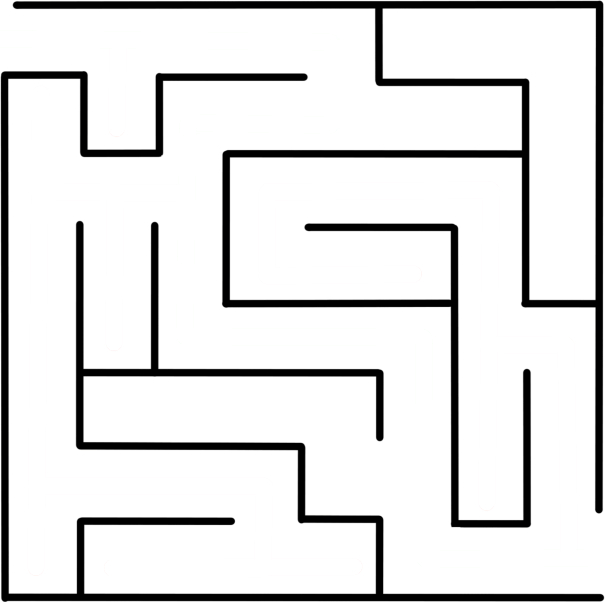
\includegraphics[width=.3\textwidth]{labirinto.jpg}
  \caption{Um exemplo de labirinto}
  \label{fig:labirinto}
\end{figure}

Resolver labirintos é uma aplicação clássica da estratégia de \emph{backtracking}, pois envolve diversas
possibilidades de caminhos e é fácil integrar \emph{checkpoints} no problema.

Imaginando que podemos traduzir a imagem acima para uma matriz onde cada ponto de decisão do
labirinto é uma célula, que todas células têm ponteiros que apontam para quatro direções: cima, baixo,
esquerda e direita, e que esses ponteiros podem levar a outras células ou ser do tipo NULL (indicando que
não há uma célula ligada naquela direção), a estratégia de backtracking pode ser usada para resolver o
problema.

\begin{algorithm}
  \caption{Backtracking}
  \begin{algorithmic}[1]
  \Procedure{find\_path}{x,y}
  \State {$\text{grid[x][y] == visited}$}
  \For{$\text{i \textbf{to} 4}$}
  \If{$\text{UP(x,y+1)}$}
  \State {$\textbf{find\_path(x,y+1)}$}
  \EndIf
  \If{$\text{LEFT(x-1,y)}$}
  \State {$\textbf{find\_path(x-1,y)}$}
  \EndIf
  \If{$\text{DOWN(x,y-1)}$}
  \State {$\textbf{find\_path(x,y-1)}$}
  \EndIf
  \If{$\text{RIGHT(x+1,y)}$}
  \State {$\textbf{find\_path(x+1,y)}$}
  \EndIf
  \EndFor
  \EndProcedure
  \end{algorithmic}
\end{algorithm}

\newpage